\documentclass{article}
\usepackage{natbib,graphicx,fullpage}
\begin{document}

\setcounter{section}{3}
\setcounter{subsection}{1}
\subsection{Reporting \textsuperscript{40}Ar/\textsuperscript{39}Ar uncertainties}
\label{sec:reportinguncertainties}

\textsuperscript{40}Ar/\textsuperscript{39}Ar dating is done by noble
gas mass spectrometry.  Argon is released from the sample in a static
ultra-high vacuum environment by heating or melting with a laser or
furnace. The released gas is first cleaned, then ionised and finally
introduced into the mass analyser.  The ion current is monitored over
regular time intervals for a duration of a few minutes. The signal
strength varies significantly during the analysis due to the competing
effects of (1) consumption of gas by the filament and (2) leakage of
additional argon from the tubing of the machine.  By convention, all
calculations are performed on the y-intercept extrapolated back to
`time zero' ($t_\circ$), i.e. the time of gas inlet. The regression of
the mass spectrometer data to $t_\circ$ is associated with statistical
uncertainty. This uncertainty is propagated down the data processing
chain, which consists of the following steps:

\begin{enumerate}
\item Blank correction: Even in the absence of sample gas, the
  collector system of the mass spectrometer will register a certain
  background current. This background signal can be measured during a
  separate `blank' run and subtracted from the measured signal.
\item Detector calibration: Until a decade ago, most noble gas mass
  spectrometers had only a single ion collector and argon measurements
  were performed by `peak hopping', i.e., by varying the magnetic
  field strength of the mass spectrometer to alternate between
  different isotopic masses. In recent years, a new generation of
  `multi-collector' noble gas mass spectrometers have been developed,
  which allow multiple isotopes to be analysed simultaneously, and the
  \textsuperscript{40}Ar/\textsuperscript{39}Ar ratio to be monitored
  directly. However the different ion detectors in a multicollector
  mass spectrometer do not necessarily respond equally to ion beams of
  equal mass and size. They can be calibrated by steering an
  appropriately sized ion beam across all the detectors and taking the
  ratio of their respective signals.
\item Mass fractionation: The five argon isotopes of interest span a
  mass range of 10\%. The sensitivity of both single- and
  multicollector instruments varies with atomic mass, and significant
  errors can occur if the resulting `mass fractionation' is
  uncorrected for. The mass fractionation factor can be quantified by
  comparing the measured \textsuperscript{40}Ar/\textsuperscript{36}Ar
  signal ratio of an air shot with its known isotopic ratio. This is
  associated with some analytic uncertainty \citep[e.g., 298.56 $\pm$
    0.31,][]{lee2006}.
\item\label{it:atmospheric} Atmospheric argon correction: Argon is a
  major consituent of the Earth's atmosphere. 0.934\% of the air that
  we breathe consists of argon, 99.6035 $\pm$ 0.0004 \%
  \textsuperscript{40}Ar, 0.3336 $\pm$ 0.0004 \%
  \textsuperscript{36}Ar and 0.0629 $\pm$ 0.0001
  \textsuperscript{38}Ar \citep{lee2006}. Despite the incompatibility
  of noble gases with the crystal structure of K-bearing silicate
  minerals, trace amounts of atmospheric argon are inevitable. This
  atmospheric `contamination' can be corrected by measuring the
  \textsuperscript{36}Ar in the sample and assuming that all of this
  is of atmospheric origin. This assumption can be verified by
  isochron regression (see item~\ref{it:isochron} below).
\item Interference correction: The
  \textsuperscript{40}Ar/\textsuperscript{39}Ar-method pairs the
  natural radioactive decay of \textsuperscript{40}K to
  \textsuperscript{40}Ar with the synthetic activation of
  \textsuperscript{39}K to \textsuperscript{39}Ar. Unfortunately,
  neutron activation produces not only \textsuperscript{39}Ar but a
  host of other Ar-isotopes as well. For example, some
  \textsuperscript{40}Ar is produced by neutron activation of
  \textsuperscript{39}K, which interferes with that produced from
  \textsuperscript{40}K; \textsuperscript{39}Ar is produced from
  \textsuperscript{42}Ca; and \textsuperscript{36}Ar from
  \textsuperscript{40}Ca and \textsuperscript{35}Cl. The relative
  importance of these interferences can be determined by analysing the
  full (\textsuperscript{36,37,38,39,40}Ar) argon isotopic composition
  of co-irradiated K-glasses and Ca-salts.
\item Decay correction: Two of the five measurable argon isotopes are
  radioactive: \textsuperscript{37}Ar \citep[t$_{1∕2} = 34.95 \pm
    0.08$ days,][]{renne2001} and \textsuperscript{39}Ar
  \citep[t$_{1∕2} = 269 \pm 3$ years,][]{stoenner1965}. A correction
  is required for the loss of these isotopes during the time elapsed
  between irradiation and analysis \citep{wijbrans1986}.
\item Interpolation of the irradiation parameter: The parameter J
  quantifying the production of \textsuperscript{39}Ar from
  \textsuperscript{39}K in the age equation is determined by analysing
  the argon composition of a co-irradiated fluence monitor with
  accurately known K-Ar age. This composition may vary across the
  irradiation stack due to neutron flux gradients in the reactor,
  which can be quantified by analysing several fluence monitors
  interspersed with the samples at known positions. The most
  appropriate J-factor for each sample is then obtained by simple
  linear interpolation.
\item\label{it:isochron} Sample averaging: The J-factors and
  radiogenic \textsuperscript{40}Ar/\textsuperscript{39}Ar-ratios
  obtained from the previous steps provide all the elements needed to
  calculate a single \textsuperscript{40}Ar/\textsuperscript{39}Ar
  age.  However it is usually beneficial to combine multiple analyses
  together to improve the precision of the dates and address their
  reproducibility. These analyses may be total fusion ages or heating
  steps in a diffusion experiment. The resulting data can be averaged
  by taking a weighted mean, or by forming an isochron. An isochron is
  obtained by omitting the atmospheric argon correction
  (step~\ref{it:atmospheric}) from the data processing chain, and
  plotting the \textsuperscript{36}Ar/\textsuperscript{40}Ar-ratio
  against the
  \textsuperscript{39}Ar/\textsuperscript{40}Ar-ratio. This results in
  a linear array of points whose horizontal and vertical intercept
  constrain the atmospheric and radiogenic argon compositions,
  respectively\footnote{This is called an `inverse' isochron. A
    `normal' isochron is formed by plotting
    \textsuperscript{40}Ar/\textsuperscript{36}Ar against
    \textsuperscript{39}Ar/\textsuperscript{36}Ar. The radiogenic
    \textsuperscript{40}Ar/\textsuperscript{39}Ar-ratio is then given
    by the slope, while the atmospheric
    \textsuperscript{40}Ar/\textsuperscript{36}Ar-ratio corresponds to
    the y-intercept.}.
\end{enumerate}

Each of the steps in the \textsuperscript{40}Ar/\textsuperscript{39}Ar
data processing chain involves statistical uncertainty.
Figure~\ref{fig:accuracyVSprecision} shows the results of a
sensitivity analysis performed at the WiscAr lab using a Nu
Instruments Noblesse multicollector mass spectrometer.  By eliminating
individual steps of the processing chain,
Figure~\ref{fig:accuracyVSprecision} reveals the relative effect of
the different corrections. These will differ for samples of different
age and composition.

\subsubsection{Random vs. systematic uncertainties}
\label{sec:randomVSsystematic}

The statistical uncertainties can be classified into two components
\citep{renne1998}:

\begin{enumerate}
  \item Random (or internal) errors can be conceptually defined as the
    natural variability that would arise if the same sample were dated
    multiple times under the same experimental conditions. These
    uncertainties originate from electronic noise in the ion
    detectors, counting statistics, temporal variability of the blank
    as a result of changes in the lab environment, etc. The
    uncertainty associated with the random errors can be quantified by
    taking replicate measurements. The standard error of these
    measurements ($\sigma/\sqrt{n}$ where $\sigma$ is the standard
    deviation of $n$ replicate measurements) is a measure of their
    \emph{precision}. The standard error can be reduced to arbitrarily
    low levels by simply averaging more measurements (i.e., by
    increasing $n$). For example, the precision of the
    t$_\circ$-intercepts can be increased by simply extending the
    duration of the noble gas measurement.
  \item Systematic (or external) errors include the systematic effects
    of decay constant uncertainty, the K/Ar ratio of the age standard,
    the air ratio etc. Getting these constants wrong causes
    \emph{bias} in some or all of the measurements and thus affects
    the \emph{accuracy} of the age determinations. In contrast with
    the random uncertainties, the systematic uncertainties cannot be
    characterised by repeat measurements, and cannot be reduced by
    simple averaging. The best way to assess the magnitude of
    systematic uncertainties is to analyse secondary standards.  These
    are materials of independently known age that are treated as
    unknowns.
\end{enumerate}

Great care must be taken which sources of uncertainty should or should
not be included in the error propagation.  Inter-sample comparisons of
\textsuperscript{40}Ar/\textsuperscript{39}Ar data may legitimately
ignore systematic uncertainties as well as all intercalibration
factors common to the dates. However, when comparing a
\textsuperscript{40}Ar/\textsuperscript{39}Ar-age with, say, a zircon
U/Pb age both random and systematic uncertainties must be accounted
for. The conventional way to tackle both types of comparisons is
called `hierarchical' error propagation \citep{renne1998, min2000}.
Under this paradigm, the random uncertainties are processed first, and
the systematic uncertainties afterwards.\\

Hierarchical error propagation is straightforward in principle but not
always in practice. Most processing steps are of a hybrid nature, with
both systematic and random uncertainties.  Consider, for example, two
samples that were analysed one month apart. In that case, the
analytical uncertainty associated with the decay correction will be
smaller for the first than the second sample. But both corrections
will be affected by the same degree of relative systematic bias.  In
an alternative approach to hierarchical error propagation,
\citet{vermeesch2015b} developed an algorithm to process the internal
and external error jointly, in matrix form. This algorithm solves the
problem with hybrid error models, but has not yet been widely adopted
by the user \textsuperscript{40}Ar/\textsuperscript{39}Ar community.

\subsubsection{Assessing goodness of fit: pitfalls and opportunities}
\label{sec:MSWD}

The random scatter of the data around an isochron or weighted mean fit
can be assessed using the Mean Square of the Weighted Deviates
\citep[MSWD,][]{mcintyre1966}. This statistic is more generally known
as the `reduced Chi-square statistic' outside geology. The MSWD is
defined as the sum of the squared differences between the observed and
the expected values, normalised by the analytical uncertainties and
divided by the degrees of freedom of the fit.  In the context of the
weighted mean age, the MSWD of $n$ age estimates is given by:

\begin{equation}
  \mathrm{MSWD} = \frac{1}{n-1} \sum\limits_{i=1}^{n} \frac{\left(x_i
    - \bar{x}\right)^2}{\sigma_i^2}
  \label{eq:MSWD}
\end{equation}

\noindent where $x_i$ is the $i$\textsuperscript{th} (out of $n$)
dates, $\sigma_i$ is the corresponding analytical uncertainty, and
$\bar{x}$ is the weighted mean of all $n$ dates. The definition for
the isochron regression is similar but involves a few more terms to
account for correlated uncertainties between the x- and y-variable.

\begin{enumerate}
\item If the analytical uncertainties $\sigma_i$ are the only source
  of scatter between the $n$ aliquots, then MSWD$\approx$1
  (Figure~\ref{fig:MSWD}a).

\item MSWD-values that are close to zero indicate that the analytical
  uncertainties have not been propagated correctly. In practice, this
  often reflects the presence of undetected error correlations. For
  example, if we propagate the J-factor uncertainty into the age
  uncertainty $\sigma_i$, then that would lower the MSWD-value. This
  is because the uncertainty of J is shared by all the $n$ age
  estimates, and this is not accounted for by Equation~\ref{eq:MSWD}
  (Figure~\ref{fig:MSWD}c).
  
\item MSWD-values that are considerably greater than one indicate that
  there is some excess scatter in the data, which cannot be explained
  by the analytical uncertainties alone. This usually reflects the
  presence of some geological \emph{dispersion}. Possible causes of
  such dispersion may be the protracted crystallisation history of a
  sample, variable degrees of inheritance, or partial loss of
  radiogenic \textsuperscript{40}Ar by thermally activated volume
  diffusion (Figure~\ref{fig:MSWD}b).
\end{enumerate}

The MSWD is the source of some confusion in the user community.  Some
believe that only datasets with MSWD$\approx$1 are suitable for
publication.  This belief is evident from the dominance of low MSWD
values in the literature.  In reality, however, there is nothing wrong
with MSWD values greater than one. In fact, high MSWD values should be
considered a good thing if they reflect the high analytical precision
of the data.  Underdispersed datasets are likely to become even more
prevalent in the future, as a result of the ever increasing resolution
of mass spectrometers \citep{phillips2013}.\\

The degree of dispersion can be formally assessed with a Chi-square
test for homogeneity. The overdispersion is `statistically
significant' of the p-value of said test falls below a pre-defined
cutoff value (typically 0.05). Unfortunately, p-values are even more
often misunderstood than MSWD values. First, it is important to
realise that p-values are sample size dependent. For example,
Figure~\ref{fig:p} compares the weighted means of two samples that
were drawn from the same normal population with a mean of 100~Ma and a
standard deviation 1~Ma and analytical uncertainties of 2~Ma.\\

The first sample (Figure~\ref{fig:p}i) contains only 10 samples and
passes the Chi-square test for sample homogeneity (MSWD=1.75,
p=0.072$>$0.05).  The second sample (Figure~\ref{fig:p}i) comprises
100 samples and has an almost identical (and, in fact, slightly lower)
MSWD as the first sample (MSWD=1.74). Despite the lower MSWD, the
p-value of the second sample is four orders of magnitude less than
that of the first sample (p=0.0000069).\\

In conclusion, any geological dataset can become `significantly'
overdispersed, provided that enough samples have been analysed.
Paraphrasing John \citet{tukey1991}, it is foolish to ask if the MSWD
equals unity. It never is -- at some decimal place.  So the question
whether or not a dataset is overdispersed is of limited scientific
interest.  It is far more useful to quantify \emph{how} dispersed it
is. There are two ways to do this.\\

A first option is to assume that the excess dispersion is
multiplicative and scales in proportion to the analytical
uncertainty. In this case, the standard error of the weighted mean or
isochron intercept may be augmented by multiplying it with the square
root of the MSWD\footnote[2]{\citet[see][for a derivation of the
    $\sqrt{\mathrm{MSWD}}$ rule, for details about the alternative
    parameterisation, and software that implements
    it.]{vermeesch2018c}}.  A second option is to parameterise the
overdispersion as an additive term and estimate it as a separate
parameter\footnotemark[\value{footnote}].\\

Although the first approach is more widely used in geochronology, the
second one is actually more useful. In this case the overdispersion
has geological significance. It may be used to estimate the degree of
heterogeneity in the inherited argon composition, or quantify the
duration of a state of partial argon retention in slowly cooled
thermal histories. It is tempting to trim an overdispersed dataset by
selectively rejecting `outliers' until p$>$0.05. However by doing so
one risks losing geologically valuable information and biasing the
results.\\

We would like to finish this section with a brief note about
\textsuperscript{40}Ar/\textsuperscript{39}Ar age spectra. These are a
useful tool to visualise stepwise heating measurements. Their
appearance is based on the weighted mean plot, with the different
heating steps arranged in order of increasing degree of degassing
along the horizontal axis, and the width of the different sample boxes
proportional to the corresponding amounts of \textsuperscript{39}Ar.
The `plateau age' is conventionally defined as the weighted mean age
of the longest sequence (in terms of cumulative \textsuperscript{39}Ar
content) of consecutive heating steps that pass the Chi-square test
for homogeneity. Note that this definition is guilty of the `cherry
picking' flaw that was discussed in the previous paragraph.  Plateau
ages should therefore only be used for qualitative purposes.

\clearpage

\begin{figure}
  
\includegraphics[width=\textwidth]{accuracyVSprecision.pdf}
  \caption{Sensitivity analysis for a single total fusion analysis of
    a $527 \pm 2 \mathrm{ka} (1\sigma)$ sanidine crystal, showing the
    effect of omitting specific steps in the data processing chain on
    the accuracy (horizontal axis) and precision (vertical axis) of
    the results. The white square in the right panel shows the best
    age estimate using all corrections.}
  \label{fig:accuracyVSprecision}
\end{figure}

\begin{figure}
  \centering
  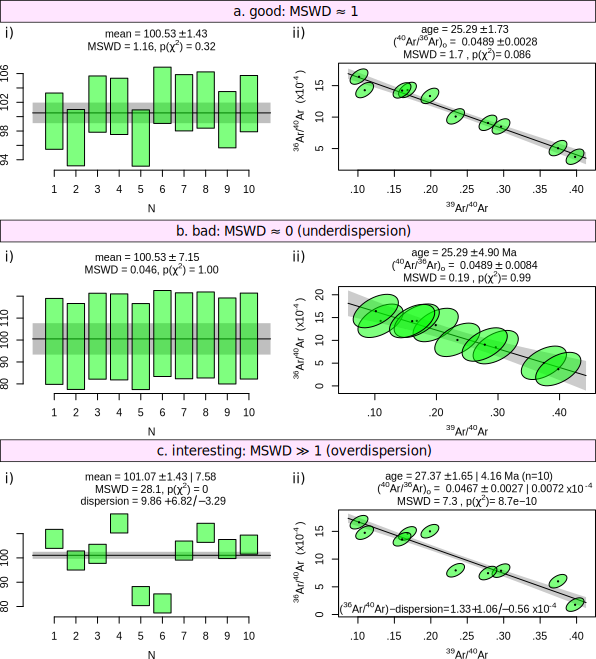
\includegraphics[height=.7\textheight]{MSWD.pdf}
  \caption{Six synthetic \textsuperscript{40}Ar/\textsuperscript{39}Ar
    datasets shown as i) weighted mean and ii) inverse isochron plots.
    The analytical uncertainties are shown as 95\% error bars and
    error ellipses, respectively. Each of the datasets consists of ten
    aliquots that are affected by a combination of analytical and
    geological dispersion.  The relative importance of these two
    sources of scatter can be assessed using the MSWD. a) If the
    analytical uncertainties alone explain the total scatter around
    the true average/trend, then the MSWD is expected to take on a
    value of around one. b) Datasets that exhibit MSWD values close to
    zero are said to be `underdispersed' with respect to the
    analytical uncertainties.  This indicates some problem with the
    error propagation, which is often due to undetected systematic
    effects.  c) Finally, MSWD values greater than one can often be
    attributed to some form of geological dispersion. This
    overdispersion carries geological significance and can be
    estimated from the data. All uncertainties are reported at 95\%
    confidence. The two age uncertainties in section c. of this plot
    are without and with overdispersion, respectively. See
    Section~\ref{sec:MSWD} of the main text for further details.}
  \label{fig:MSWD}
\end{figure}

\begin{figure}
  \centering
  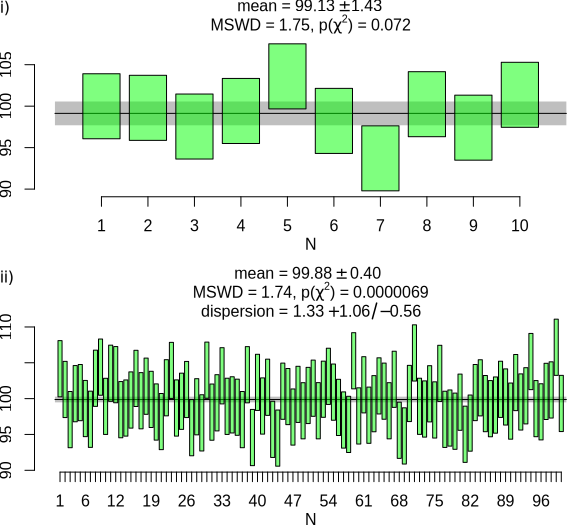
\includegraphics[height=.6\textwidth]{p.pdf}
  \caption{Two random samples drawn from the same synthetic
    population, which is characterised by 2~Ma analytical
    uncertainties (1$\sigma$) and 1\% geological dispersion. i) A
    small ($n = 10$) dataset is insufficient to detect the dispersion
    ($p < 0.05$). ii) A ten-fold increasing in sample size (to
    $n=100$) greatly increases the power of the Chi-square test.  This
    results in a much lower p-value than for the small dataset,
    despite the slightly lower MSWD value. Conclusion: p-values are
    sample size dependent and should not be used as a measure of
    overdispersion. Instead, it is more productive to estimate the
    dispersion from the data. Doing so for the large sample yields a
    dispersion estimate of 1.33~Ma with an (asymmetric) confidence
    interval of +1.06/-0.56~Ma.}
  \label{fig:p}
\end{figure}

\clearpage

\bibliographystyle{/home/pvermees/Dropbox/abbrvplainnat}
\bibliography{/home/pvermees/Dropbox/biblio}

\end{document}
